\documentclass[a4paper, 10pt]{article}

\usepackage[margin=2cm]{geometry}
\usepackage{hyperref}
\usepackage{graphicx}

\begin{document}
\begin{center}
\begin{tabular}{ p{10cm} p{10cm} }
& +91 91 4594 6493 \\ 
{\textbf{\LARGE{Hemant Goraksh Ghuge}}} &\href{mailto:hemantgghuge@gmail.com}{hemantgghuge@gmail.com} \\ 
&\url{in.linkedin.com/in/hemant-ghuge} \\ &\url{hemantghuge.wordpress.com} \\ 
&\url{github.com/HemantGorakshGhuge}
\end{tabular}
\end{center}
\vspace{-0.7cm}
\begin{center}
\line(1,0){500}
\end{center}

%\begin{figure}[h]
%\centering
%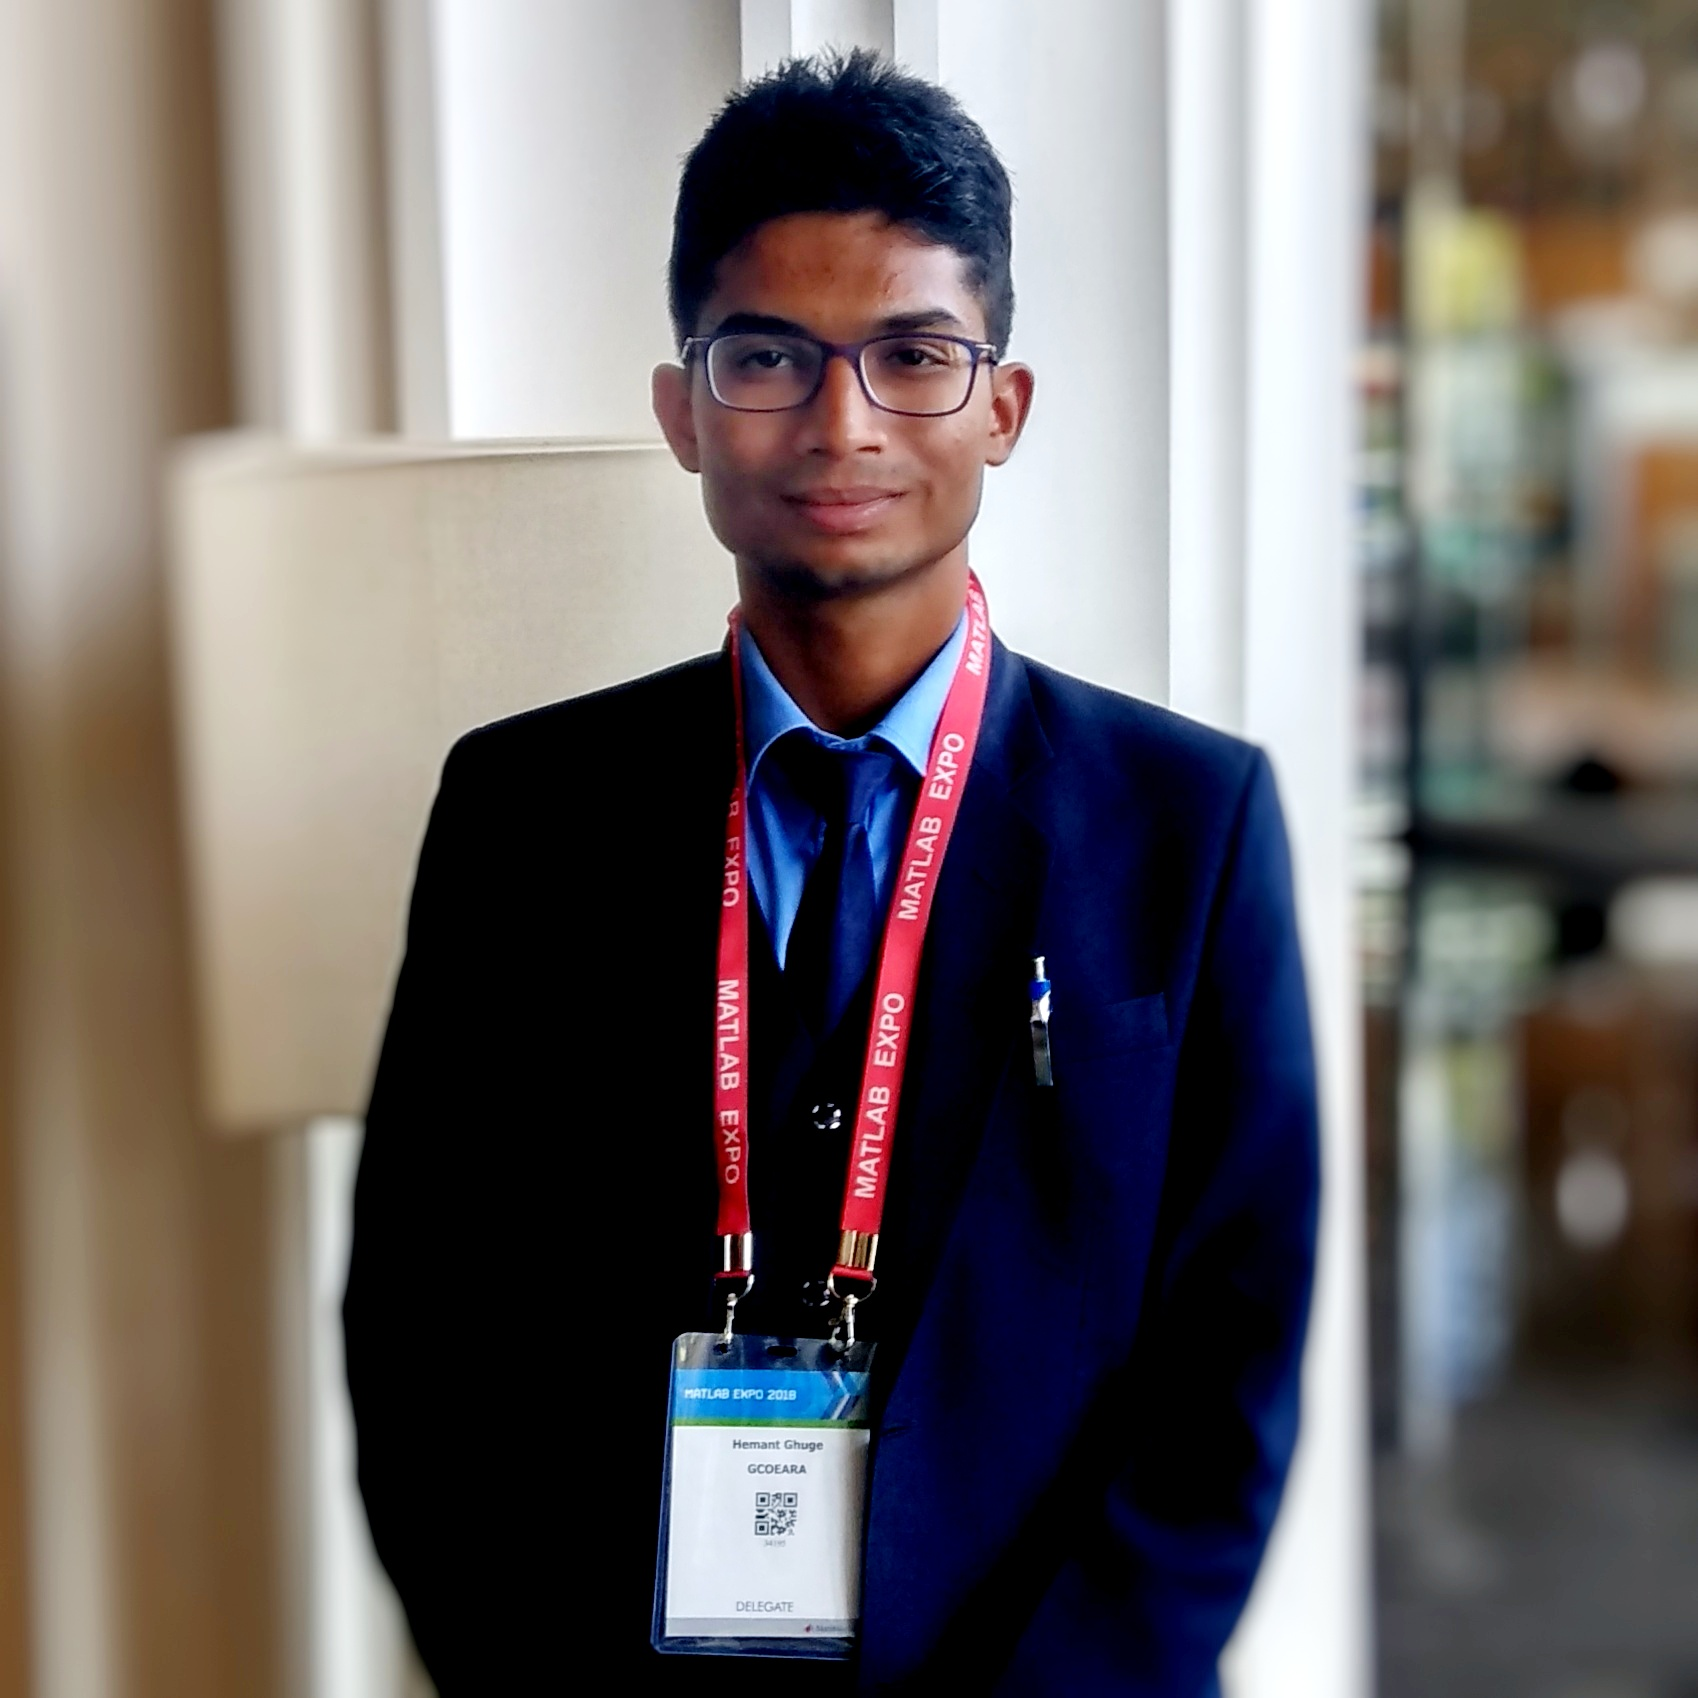
\includegraphics[width=5cm, angle=0]{ResumePhoto.jpg}
%\end{figure}

{\textbf{\Large{OBJECTIVE:}}}\\

To pursue a challenging career and be part of a progressive organisation that presents scope to enhance my knowledge, creativity utilizing my skill toward the development of the organization.\\

{\textbf{\Large{EDUCATION:}}}\\

\vspace{-0.7cm}
\begin{center}
\begin{tabular}{|c|c|c|c|c|}
\hline
\textbf{EXAM} & \textbf{COLLEGE/SCHOOL} & \textbf{BOARD} & \textbf{YEAR} & \textbf{AGGREGATE}\\ \hline 
B.E ENTC & Government College of Engineering and Research &  S.P.P.U & 2020 & 7.67 (Till 7th Sem)\\ \hline
H.S.C & Army Public School, Mumbai & C.B.S.E & 2016 & 82.8\\ \hline
S.S.C & Army Public School, Mumbai & C.B.S.E & 2014 & 8.8\\ \hline
\end{tabular}
\end{center}

{\textbf{\Large{PROJECTS:}}}
\begin{itemize}
\item {\textbf{\large{Smart and Efficient Techniques for Automated Guided Vehicle}}}

Presently our BE project team is working on AGV (Automated Guided Vehicle) which is \textbf{Tri-Wheel Omni} based vehicle$.$ A self-developed \textbf{PCB} is used instead of complex circuitry and the AGV is controlled with a \textbf{custom GUI} developed by the team for task planning$.$ %\textbf{Self-Charging} and \textbf{Power Management} are one of the key feature of our project$.$ 

\item {\textbf{\large{MathWorks MiniDrone Competition}}}

Designed a line follower and \textbf{angle estimation algorithm} for a Mini-Drone using Control System and Computer Vision Toolbox. It includes \textbf{Model-Based Design} using Simulink. We have \textbf{secured 5th} among the shortlisted teams from across India, at the National Finals of the MathWorks Minidrone competition held at NUMA Bengaluru.

\item {\textbf{\large{National DD Robocon 2019}}}

Designed and built a Four Mecanum Wheeled Omnidirectional Mobile Robot and a Quadruped Robot (Automatic) using 8 BLDC motors for the competition$.$ We used Image processing for the navigation of Quadruped Robot$.$ The team secured \textbf{AIR 4th} and won \textbf{Special Jury Award}.

\item {\textbf{\large{Fire Rescue System (FRS) for High-Rise Building}}}

FRS is a secondary evacuation system used during fire accidents$.$ With this project, our team was selected as one of the \textbf{21 finalists out of 362 teams} in eYantra Ideas Competition held at IIT Bombay and demonstrated our project at National Finals and Symposium 2019.

%\item {\textbf{\large{In-House Mechatronics Kit(33 in 1)}}}

%The kit is a custom PCB which covers \textbf{33 experiments} of SPPU syllabus of \textbf{4 branches}. It comes under college development projects.

\item {\textbf{\large{National Robotic Contest Robocon 2018}}}

Designed and built Tri-Omni Wheeled Omnidirectional Mobile Robot and four Mecanum Wheeled Omnidirectional Mobile Robot$.$ Rack picking and Shuttlecock throwing mechanism were also designed and implemented$.$ The 2nd fastest team to complete the task$.$ \\
\textbf{AIR 2nd (League Matches)} and won \textbf{Smart and Simple Robot Award} by Robu.in with a cash prize worth 50k.

\item {\textbf{\large{ServoEyePi}}}

\textbf{Raspberry Pi} based Computer Vision project using servo motor and pi cam with \textbf{MATLAB} programming$.$ The project was awarded as \textbf{Innovative Project} in Robo-X event - Abinitio 2018-19 (Technical Event)
%\item {\textbf{\large{UltraLine03}}}

%Arduino based obstacle avoidance and line following robot which travelled automatic zone of \textbf{ABU ROBOCON 2018} theme.
%\item {\textbf{\large{AlexaPiBhima}}}

%Raspberry Pi running amazon's "Alexa voice services"$.$ \textbf{Python} and \textbf{Bash Scripting} were used in this project.\\

\end{itemize}

{\textbf{\Large{TECHNICAL SKILLS:}}}
%\begin{itemize}
%\item MATLAB
%\item Simulink
%\item C \& Python
%\item Raspberry Pi
%\item Arduino
%\item IoT
%\item Bash Script
%\item Ubuntu
%\item Vim Text Editor
%\item Computer Vision
%\item Deep Learning \\
%\end{itemize}
\\
\begin{tabular}{p{1cm}p{3.5cm}p{3.5cm}p{3.5cm}p{3.5cm}}
\\
& Python & C & MATLAB & Simulink\\
& Raspberry Pi & Arduino & Machine Learning & Deep Learning\\
& Computer Vision & Ubuntu & Vim Text Editor & Shell Scripting\\
\\
\end{tabular}
\newpage
{\textbf{\Large{EXTRA-CURRICULAR ACTIVITIES:}}}
\begin{itemize}
\item \textbf{Senior Team Member at Robotics Research Lab, GCOEARA}

Participated in National Robotic Contest DD-Robocon 2019 and secured AIR 4 along with Special Jury Award$.$ Our team was AIR 2nd (League Table) in National Robotic Contest Robocon 2018$.$ We explore new things for the lab and endeavour to execute in the Lab.

\item \textbf{Senior Member at eLSI'19}

We the senior members of eLSI lab work for developing technical skills among other members.
\item \textbf{State Level Football Goalkeeper and Athlete}

Presently I am goal-keeper of Junnar Taluka Football Club (JTFC)$.$ Our team awarded as 2nd Runner-up in 7 a side football championship trophy 2018$.$ Participated 3 times in CBSE Cluster Football as well as Athletic Meet$.$ I was the Sports Captain of Army Public School, Mumbai. 
%\item \textbf{Typing Speed 35wpm}

%I have too craze in keyboard typing$.$ This craziness made me the winner of typing event at GPA.
\item \textbf{Rubik's Cube Solver}

Solving Rubik's Cube is one of my hobbies$.$ This hobby helped me in securing 2nd place in Rubik's Cube event at GPA. Best Time:- 53 sec\\

\end{itemize}

{\textbf{\Large{CO-CURRICULAR ACTIVITIES:}}}
\begin{itemize}
\item \textbf{SAAGA 2K18}

Member of Student Alumni Association of GCOEARA.
\item \textbf{Workshop}

Conducted and organized many workshops in college on MATLAB, and Raspberry Pi. Each time we received a great response from students.
\item \textbf{Abinito (Technical Event)}

Department Head - Abinitio 2018-19.\\
Sub-Coordinator of Line Tracing Event - Abinitio 2017-18.\\ 
%\item \textbf{Resonance (Cultural Event)} 

%Branch Theme Winner - Resonance 2017. \\
%Street-play event Winner - Resonance 2017.\\
%\item \textbf{Combat (Sports Event)}

%Football Competition Winner - Combat 2017. \\
\end{itemize}

{\textbf{\Large{TRAINING \& INTERNSHIP:}}}
\begin{itemize}
%\item I am \textbf{MATLAB Developer Intern} at MATLAB Helper. 4-month internship ending at Dec 19.
\item MATLAB, Simulink and Deep Learning Onramp training course by MathWorks
\item Drone Making Workshop organised by MindSpark Team (C.O.E.P)
\item First Aid and Life Saving Course conducted under the aegis of Headquarters Southern Command (Medical)\\
\end{itemize}

{\textbf{\Large{RESEARCH PUBLICATION:}}}
\begin{itemize}
\item A research paper on ``Fire Rescue System for High Rise Building" is presented in \textbf{5th IEEE International Conference On Computing, Communication, Control And Automation(ICCUBEA) 2019}. We won \textbf{Best Paper Award}. Soon, it will be published in IEEE Xplore.
\item A research paper on ``An Algorithm for Skew Angle Estimation and it's Application Domain" is presented in \textbf{International Conference on Signal \& Data Processing - ICSDP 2019} on 15th - 16th  November, 2019. All presented papers will be published in the prestigious Lecture Notes in Electrical Engineering (\textbf{Springer}).
\item A research paper on ``Design and Control of Quadruped Robot along with Machine Vision based Path Planning." is accepted for the oral presentation in \textbf{IEEE PuneCon} on 18th-20th December, 2019. All accepted paper will be submitted to IEEE Xplore.\\
\end{itemize}

{\textbf{\Large{PERSONAL DETAILS:}}}\\

\begin{tabular}{ p{3cm} p{6cm} p{3cm} p{6cm} }
Father's Name: & Hav$.$ Goraksh Karbhari Ghuge(Retd.) & Mother's Name: & Aruna Goraksh Ghuge \\ 
Sex: & Male & Date of Birth: & January 30, 1999\\     
Nationality: & Indian &Marital Status: & Single \\ 
\\
\end{tabular}
%{\textbf{\Large{REFERENCES}}}\\

%\begin{tabular}{ p{5cm} p{5.5cm} p{5.5cm} }
%Dr$.$ Veer Alakshendra & Dr$.$ Avinash Pant (Principal) & Dr$.$ Manoj Nagmode\\ 
%Technical Evangelist & Govt$.$ College of Engg$.$ \& Research & Head, Department of E\&TC \\      
%MathWorks & Former Vice Chairman at A.I.C.T.E & Govt$.$ College of Engg$.$ \& Research \\      
%8446985971 & 9958411661 & 9226771488 \\ 
%Veer.Alakshendra@mathworks.in & pantavinash@hotmail.com & manoj.nagmode@gmail.com \\
%\\
%\end{tabular}

{\textbf{\Large{DECLARATION}}}\\

\centerline{I hereby declare that the above-written particulars are true to the best of my knowledge and belief.}

%\vspace{0.4cm}
%{\textbf{\Large{DATE}}}\\
%\today
\end{document}
